\section{Smooth Obstacles}
The step-avoiding route shown in Figure 2 is only one example among a family of routes with equal cost. A smoothly-varying obstacle breaks this degeneracy and determines a finite number of optimal paths.

By smoothly-varying, we mean that the derivative of $f$ is defined everywhere. One such example, commonly used to model obstacles, is the Gaussian.

\begin{equation}
f(x, y) = A \exp\left(-\displaystyle\frac{x^2+y^2}{2\sigma^2}\right)
\end{equation}

The Gaussian is radially symmetric, and it decreases monotonically from its center. Both properties are sensible ones for modeling a simple obstacle.

Restricted rook-like motion in our 4-connected space, we can immediately see that any lateral steps should  be taken at the edges of the space, as far the origin as possible. For any choice of parameters, the optimal path is bracket-shaped: from $(-n,0)$ to $(-n, \yhat)$ to $(n, \yhat)$ to $(n,0)$ for some $\yhat$. (Or, equivalently, the mirror image: $y \rightarrow -y$.) Note that a direct path qualifies as a bracket with $\yhat=0$.

For the step obstacle in the previous section, the best path was determined by relative size $h/w$ and relative cost $A/P$. We might have predicted as much from dimensional analysis. In the current case, the important parameters will be $A/P$ and $\sigma/n$, the width of the Gaussian relative the distance from start to finish. We seek a relationship between these model parameters and $\yhat$, the distance of closest approach.


\begin{figure}
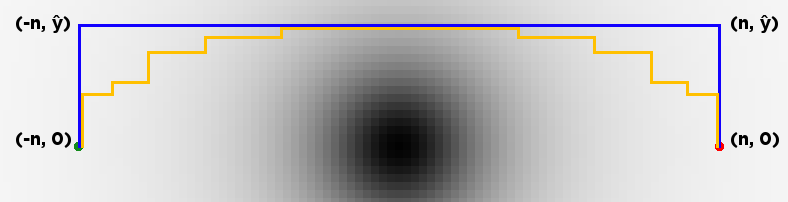
\includegraphics[width=\columnwidth]{graphix/bracket.png}
\caption{The Bracket Shape}
\label{fig:bracket}
\end{figure}